%===================================================
\chapter{Similarity Curvature Experiments}

\begin{Abstract}
In this chapter we further develop our new scale invariant curvature measure, similarity curvature. An estimator for the similarity curvature of digital surfaces is presented. Experiments and results applying similarity curvature to synthetic data are also presented.\\
\end{Abstract}

%===================================================
\section{Introduction}
Recall, from Part 1, that similarity curvature is well-motivated by numerous well known practical 3D shape applications in computer vision including 3D scan matching, alignment and merging, 3D object matching, and 3D object classification and recognition. 3D object databases are also an active research area; see, for example, \cite{Bustos_2005_FBSS}, \cite{Ichida_2004_IR3DM} and \cite{Assfalg_2004_R3DVS}.\\

We generally seek \emph{invariant} properties when characterizing 3D objects. Any characterization that is rotation, translation and scaling invariant enables determining the equivalence of shapes independent of size. Again, as mentioned in Part 1, scale invariance would also enable the use of uncalibrated measurement units in 3D digitization (e.g. scanning).\\

%===================================================
\subsection{Curvatures}
Recall that a number of different curvature measures are defined in differential geometry 
and that curvature is well defined for continuously differentiable lines and surfaces 
\cite{Davies_1996_CGCS}. Planar lines have only a single curvature measure whilst surfaces 
have a number of curvature measures, all of which are based on \emph{normal curvature}.\\

As given in Chapter~\ref{chap:curvature}, on surfaces, the two principal curvatures are
$\kappa_1$ and $\kappa_2$, where $\kappa_1$ is the maximum normal curvature
and $\kappa_2$ is the minimum normal curvature at a given point.\\

And, again, historically, the mean curvature has been given as
\begin{equation}
H = (\kappa_1 + \kappa_2)/2
\label{eq:invariant-H}
\end{equation}

and the Gaussian curvature given as
\begin{equation}
K = \kappa_1 \kappa_2
\label{eq:invariant-K}
\end{equation}

Note that, more recently, additional surface curvature measures have appeared. In \cite{Jagann_2007_3DSMS} for example, the curvature measure \emph{curvedness} has been defined as
\begin{equation}
C = \sqrt{(\kappa_1^2 + \kappa_2^2)/2}
\end{equation}

None of the above curvature measures are scale invariant. Also, recall that, with digital data, there is inherent discontinuity and curvature can only be estimated.\\

%===================================================
\section{A Similarity Curvature Estimator}
From Section~\ref{sec:curvature-similarity}, similarity curvature is, by definition,
determined by the principal curvatures. But, because a digitization acquisition pattern
will not, in general, align with the principal curvature directions, we cannot directly
compute the principal curvatures. However, recall, from
Section~\ref{sec:estimators-umbrella} and Section~\ref{sec:estimators-cut}, that we do
already have estimators for mean and Gaussian curvature.\\

Building on this previous work, similarity curvature is estimated using the following process. First the mean and Gaussian curvatures are estimated, then the principal curvatures are calculated from the mean and Gaussian curvatures as follows:
\begin{equation}
\tilde{\kappa}_1 = \tilde{H} + \sqrt{\tilde{H}^2 - \tilde{K}}
\label{eq:invariant-k1}
\end{equation}
\begin{equation}
\tilde{\kappa}_2 = \tilde{H} - \sqrt{\tilde{H}^2 - \tilde{K}}
\label{eq:invariant-k2}
\end{equation}
Finally, the (estimated) similarity curvature is calculated from these principal curvatures
using Definition~\ref{def:curvature-similarity1} and
Definition~\ref{def:curvature-similarity2} as was given in
Section~\ref{sec:curvature-similarity}.\\

Equations~(\ref{eq:invariant-k1}) and (\ref{eq:invariant-k2}) are easily verified. Substitution using Equations~(\ref{eq:invariant-H}) and (\ref{eq:invariant-K}) gives
\begin{align}
H + \sqrt{H^2 - K} &= \Bigl(\frac{\kappa_1 + \kappa_2}{2}\Bigr) + \sqrt{\Bigl({\frac{\kappa_1 + \kappa_2}{2}}\Bigr)^2 - \kappa_1 \kappa_2}\\
&= \Bigl(\frac{\kappa_1 + \kappa_2}{2}\Bigr) + \sqrt{\Bigl({\frac{\kappa_1^2 + 2\kappa_1\kappa_2 + \kappa_2^2}{4}}\Bigr) - \Bigl(\frac{4\kappa_1 \kappa_2}{4}\Bigr)}\\
&= \Bigl(\frac{\kappa_1 + \kappa_2}{2}\Bigr) + \sqrt{\Bigl(\frac{\kappa_1^2 - 2\kappa_1\kappa_2 + \kappa_2^2}{4}\Bigr)}\\
&= \Bigl(\frac{\kappa_1 + \kappa_2}{2}\Bigr) + \Bigl(\frac{\kappa_1 - \kappa_2}{2}\Bigr)\\
&= \frac{\kappa_1}{2} + \frac{\kappa_2}{2} + \frac{\kappa_1}{2} - \frac{\kappa_2}{2} = \kappa_1
\end{align}
and
\begin{align}
H - \sqrt{H^2 - K} &= \Bigl(\frac{\kappa_1 + \kappa_2}{2}\Bigr) - \sqrt{\Bigl({\frac{\kappa_1 + \kappa_2}{2}}\Bigr)^2 - \kappa_1 \kappa_2}\\
&= \Bigl(\frac{\kappa_1 + \kappa_2}{2}\Bigr) - \sqrt{\Bigl({\frac{\kappa_1^2 + 2\kappa_1\kappa_2 + \kappa_2^2}{4}}\Bigr) - \Bigl(\frac{4\kappa_1 \kappa_2}{4}\Bigr)}\\
&= \Bigl(\frac{\kappa_1 + \kappa_2}{2}\Bigr) - \sqrt{\Bigl(\frac{\kappa_1^2 - 2\kappa_1\kappa_2 + \kappa_2^2}{4}\Bigr)}\\
&= \Bigl(\frac{\kappa_1 + \kappa_2}{2}\Bigr) - \Bigl(\frac{\kappa_1 - \kappa_2}{2}\Bigr)\\
&= \frac{\kappa_1}{2} + \frac{\kappa_2}{2} - \frac{\kappa_1}{2} + \frac{\kappa_2}{2} = \kappa_2
\end{align}

In this chapter, we have chosen (somewhat arbitrarily) to employ the triangle umbrella mean and triangle umbrella Gaussian curvature estimators. Recall that the Gaussian curvature is estimated by
\begin{equation*}
\tilde{K} = \frac{3(2\pi-\sum{\alpha_n})}{\sum{{\cal A}(f_n)}}
\end{equation*}
and mean curvature is estimated by
\begin{equation*}
\tilde{H} = \frac{3 \sum{\beta_n \, ||e_n||}}{4 \sum{{\cal A}(f_n)}}
\end{equation*}

%===================================================
\section{Experiments}

\begin{figure}[!t]
\begin{center}
\epsfig{file=chapters/Invariant/scan_grid, height=48mm}
\end{center}
\vspace{-20pt}
\caption{Scan grid.}
\label{fig:invariant-scan}
\end{figure}
Synthetic digital data has been created for a number of simple and compound objects. Each object was digitized by orthogonally scanning from above (in simulation) using the offset rasterization pattern shown in Figure~\ref{fig:invariant-scan}(a), which results in 6-neighborhood (hexagonal) point adjacency as shown in Figure~\ref{fig:invariant-scan}(b). The scan grid has a \emph{pitch} dimension as illustrated in the same Figure. Note that, with this scanning method, only the portion of an object which faces towards the scanning source direction gets digitized.\\

%===================================================
\subsection{Similarity Curvature Histograms}

Experimental reference shapes included a sphere, cylinder, ellipsoid and torus. To evaluate
the similarity curvature estimation, we considered each reference shape in turn with an
initial scan pitch of 1.0, then a 10x scaling, and finally a 10x scan resolution. For the
10x scaling, both the scan pitch and the object size were increased by a factor of ten. For
the 10x resolution, the scan pitch was decreased by a factor of ten and the initial object
size was retained. Of course, this finer scan pitch increases the total number of scan
points by a factor of approximately 100x.\\

Initial object sizes where chosen such that the resultant number of digitized points was somewhere in the range of sixty to one hundred. Subsequently, of course, the 10x scan resolution resulted in digitized point counts that were more than one hundred times greater.\\

Similarity curvature values where calculated at each scanned object point. Recall, from Section~\ref{sec:curvature-similarity-space}, that similarity curvature values can be uniquely placed on $e$-axis and $h$-axis positions in the similarity curvature space.\\

In this first analysis, the resultant similarity curvature values have been accumulated for summary in associated $e$-axis and $h$-axis histograms. Consistent with common practice, curvature values are indicated on each horizontal axis and point counts are indicated on each vertical axis.\\

\begin{figure}[!t]
\begin{center}
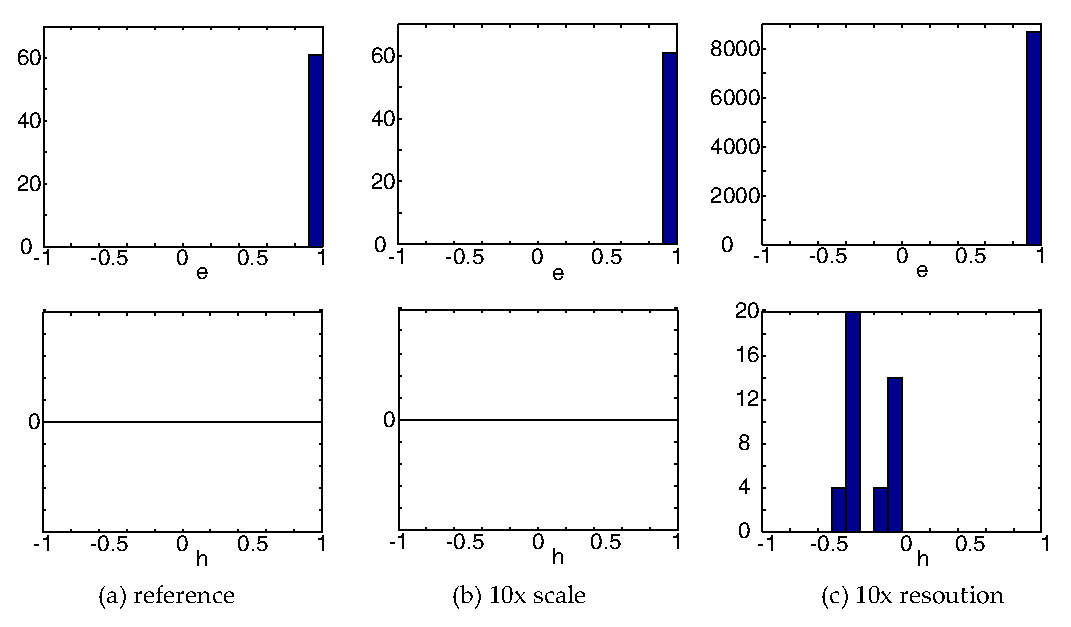
\epsfig{file=chapters/Invariant/s_eh, width=128mm}
\end{center}
\vspace{-10pt}
\caption{Sphere $eh$-histograms for reference, 10x scale, 10x resolution.}
\label{fig-s}
\end{figure}
Sphere results are shown in Figure \ref{fig-s}. The reference sphere that was used has a radius of 5. Observe that the similarity curvature has the constant value of 1 in the $e$ histograms regardless of scale. For a sphere, we would not expect any $h$-axis values. However, due to limited precision arithmetic, there are a small number (approximately 0.5 percent of the total count) of erroneous values in the high resolution $h$ histogram.\\

\begin{figure}[!t]
\begin{center}
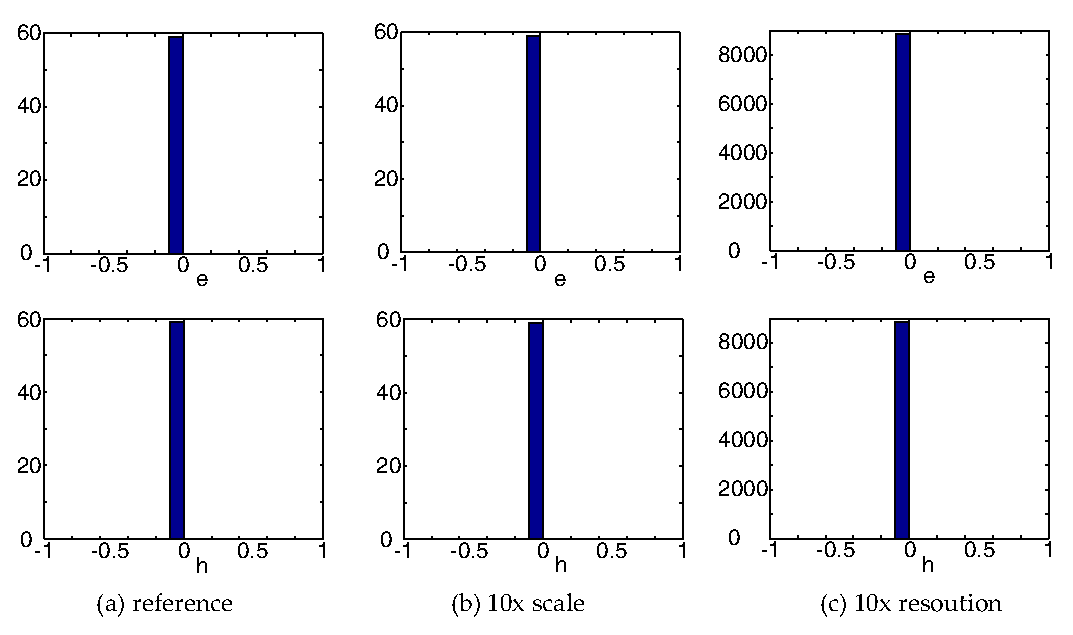
\epsfig{file=chapters/Invariant/c_eh, width=128mm}
\end{center}
\vspace{-10pt}
\caption{Cylinder $eh$-histograms for reference, 10x scale, 10x resolution.}
\label{fig-c}
\end{figure}
Cylinder results are shown in Figure \ref{fig-c}. The reference cylinder that was used has
a radius of 5 and a height of 4. As expected, in all cases the $e$ and $h$ values are
constant at zero. Recall that this zero similarity is expected whenever the Gaussian
curvature is zero, as is the case for a cylinder.\\

\begin{figure}[!t]
\vspace{10pt}
\begin{center}
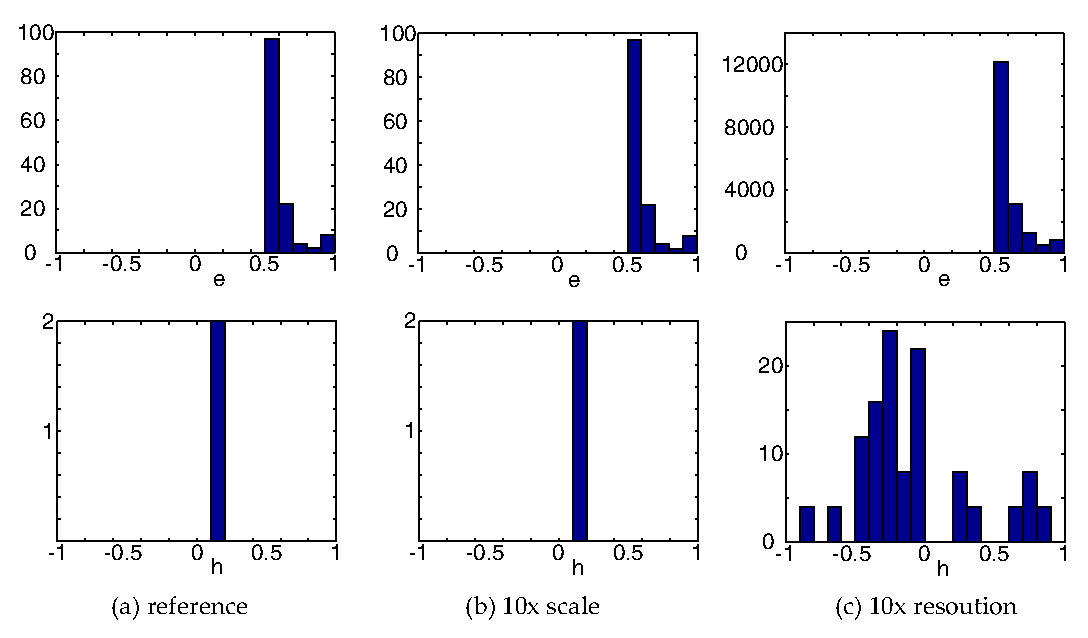
\epsfig{file=chapters/Invariant/e_eh, width=128mm}
\end{center}
\vspace{-10pt}
\caption{Ellipsoid $eh$-histograms for reference, 10x scale, 10x resolution.}
\label{fig-e}
\end{figure}
Ellipsoid results are shown in Figure \ref{fig-e}. The reference ellipsoid that was used has axes equal to 6 and 12. As expected, the $e$ values are bounded by 1 and $(1/12)/(1/6)=0.5$. As was the case for a sphere, we would not expect any $h$-axis similarity curvature values for an ellipsoid. However, again due to finite precision arithmetic, this time an error count equal to approximately 2 percent of the total number of points has accumulated in each of the $h$ histograms.\\

\begin{figure}[!t]
\begin{center}
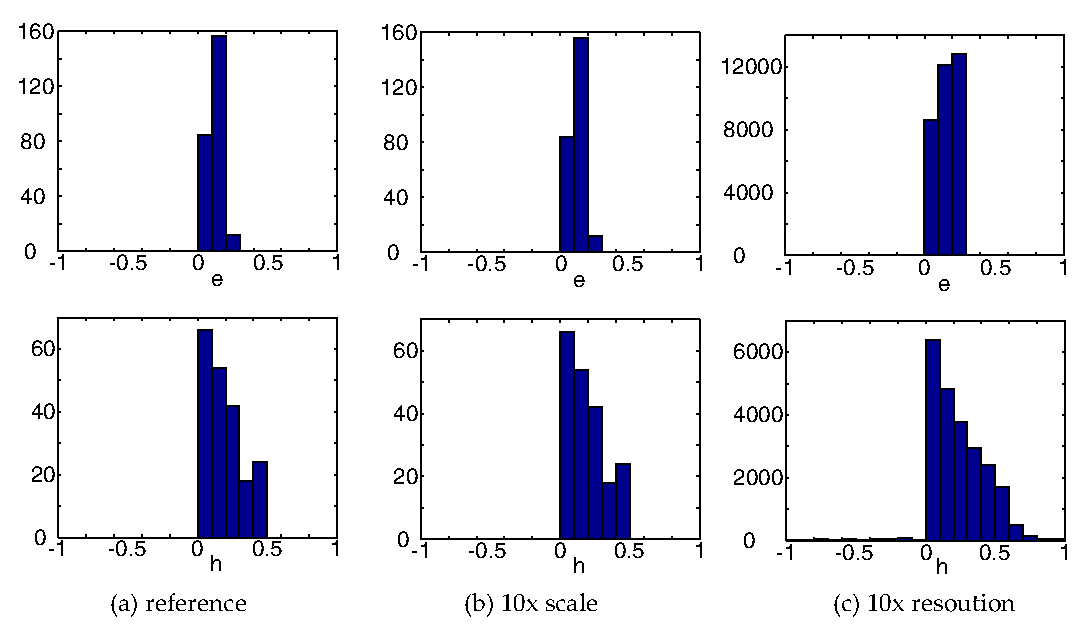
\epsfig{file=chapters/Invariant/t_eh, width=128mm}
\end{center}
\vspace{-10pt}
\caption{Torus $eh$-histograms for reference, 10x scale, 10x resolution.}
\label{fig-t}
\end{figure}
Torus results are shown in Figure \ref{fig-t}. The reference torus that was used has an inner radius of 6 and an outer radius of 14, which implies an interior radius of $(14-6)/2=4$. As expected, based on the associated minimum and maximum curvatures of $1/14$ and $1/4$ respectively along the outer circumference, the $e$ values are bounded by 0 and $(1/14)/(1/4)\approx0.29$. The associated minimum and maximum curvatures of $1/6$ and $1/4$ respectively along the inner circumference, result in $h$ values which are bounded by 0 and $(1/6)/(1/4)\approx0.67$.\\

%===================================================
\subsection{Shading Coded Similarity Curvature}

\begin{figure}[!t]
\begin{center}
\epsfig{file=chapters/Invariant/EH-shading, height=50mm}
\end{center}
\vspace{-15pt}
\caption{Shading coded $eh$-axis.}
\label{fig:EH-shading}
\end{figure}
In this section we assign color coding to similarity curvature values as was done in Section~\ref{sec:curvature-visualization}. An example color coding scheme for the $eh$-plot axis is shown in Figure \ref{fig:EH-shading} where negative $e$ values are pure green, positive $e$ values are pure red, negative $h$ values are pure blue and positive $h$ values are pure yellow. These similarity curvature shading coded values can be used to color each surface point on test objects for visualization purposes.\\

\begin{figure}[!t]
\begin{center}
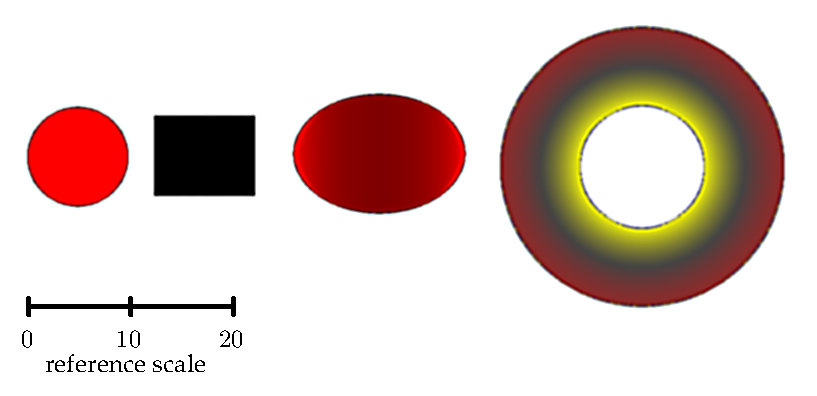
\epsfig{file=chapters/Invariant/shading_coded_BLUR, height=45mm}
\end{center}
\vspace{-10pt}
\caption{Shading coded similarity curvature reference images: sphere, cylinder, ellipsoid, torus.}
\label{fig:shading-coded}
\end{figure}
Shading coded similarity curvature images for each of the test reference shapes used in the previous section are shown in Figure \ref{fig:shading-coded}. The constant curvature of the sphere and the cylinder as well as the smooth transition through curvature values in the curvature maps of the ellipsoid and the torus are readily apparent.\\

\begin{figure}[!t]
\begin{center}
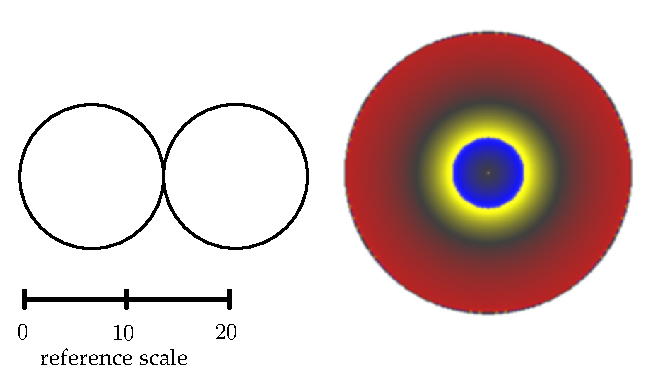
\epsfig{file=chapters/Invariant/torus_BLUR, height=50mm}
\end{center}
\vspace{-12pt}
\caption{Torus cross section and shading coded similarity curvature image.}
\label{fig-torus}
\end{figure}
Figure \ref{fig-torus} shows the case of a torus having an inner radius of zero. Note the $h$-axis wrapping near the center of the torus. The bright yellow color transitions change abruptly to bright blue when the $h$-axis similarity curvature wraps around, changing sign.\\

%===================================================
\subsection{3D Object Detection}
Similarity curvature can be used to identify and extract 3D shapes from within complex 3D
scan scenes. We may wish to, for example, identify all (convex) spheres and spherical patches within
a scene no matter what the sphere size or scan resolution.\\

We have constructed a test scan scene containing a surface with five each spherical, ellipsoid and toroid bumps, as well as five pits each having those same shapes, with some of the pits and bumps overlapping. Several representations of the scene are shown in Figure~\ref{fig-surface}. Figure~\ref{fig-surface}(a) is a shading coded depth image in which points closer to the scan source are white color shaded, and more distant points are shaded black. A color coded similarity curvature image is shown in Figure~\ref{fig-surface}(b), in which spherical bumps are pure red and spherical pits are pure green. Finally, all of the spherical bump surface patches have been identified and color coded as white in Figure~\ref{fig-surface}(c).

\begin{figure}[!t]
\begin{center}
\epsfig{file=chapters/Invariant/surface_maps, width=110mm}
\end{center}
\vspace{-12pt}
\caption{Color shaded test scene images illustrating (a) depth, (b) curvature, (c) extracted spherical patches.}
\label{fig-surface}
\end{figure}
